\documentclass[11pt,fleqn]{article}
%\usepackage{CJK}
\usepackage{latexsym}
\usepackage{color}
\usepackage{graphicx, float}\usepackage{graphicx}
%\usepackage[colorlinks]{hyperref}
\setlength{\oddsidemargin}{-0.0in}
\setlength{\evensidemargin}{-0.0in} \setlength{\textwidth}{6.0in}
\setlength{\textheight}{9.0in} \setlength{\topmargin}{-0.2in}

%\setlength{\leftmargin}{0.7in}
\usepackage{amssymb, graphicx, amsmath}  %  fancyheadings,

\newcommand\qed{\qquad $\square$}
\newcommand{\nn}{\nonumber}

\def \[{\begin{equation}}
\def \]{\end{equation}}
\def\proof{{\bf Proof:\quad}}
\def \endzm {\quad $\Box$}
\def\dist{\hbox{dist}}


\newcommand{\R}{\mathbb{R}}
%\newtheorem{yinli}{����}[section]
\newcommand{\D}{\displaystyle}
\newcommand{\T}{\textstyle}
\newcommand{\SC}{\scriptstyle}
\newcommand{\FT}{\footnotesize}



%\newtheorem{theorem}{Theorem}[section]
%\renewcommand{\thetheorem}{\arabic{section}.\arabic{theorem}}
\newtheorem{definition}{Definition}
\renewcommand{\thedefinition}{\arabic{section}.\arabic{definition}}
\newtheorem{lemma}{Lemma}[section]
\renewcommand{\thelemma}{\arabic{section}.\arabic{lemma}}
\newtheorem{remark}{Remark}
\renewcommand{\theremark}{\arabic{section}.\arabic{remark}}
\newtheorem{proposition}{Proposition}[section]
\renewcommand{\theproposition}{\arabic{section}.\arabic{proposition}}
\newtheorem{corollary}{Corollary }[section]
\renewcommand{\thecorollary}{\arabic{section}.\arabic{corollary}}
\renewcommand{\theequation}{\arabic{section}.\arabic{equation}}
\renewcommand{\baselinestretch}{1.35}
\newtheorem{exam}{Example}[section]
\renewcommand{\theexam}{\arabic{section}.\arabic{exam}}
\newtheorem{theo}{Theorem}[section]
\renewcommand{\thetheo}{\arabic{section}.\arabic{theo}}
\begin{document}
%\begin{CJK*}{GBK}{song}

\begin{center}

{\LARGE \bf  Machine Learning and Computer Vision Assignment 1}\\


\vskip 15pt
 {Huihuang Zheng, huihuang@utexas.edu }\\
\vskip 5pt
{\small hz4674 Fall 2015 }


\end{center}

\section{Part I, Short Answer Problems}
\begin{enumerate}
  \item Suppose we have filter $f_1 \in \mathbb{R}^{1 \times n}$, $f_2 \in \mathbb{R}^{n \times 1}$. We have convolution $f_1 * f_2 \in \mathbb{R}^{n \times n}$. Suppose we have a picture $g$ of $k \times m$ pixels. Time complexity of performing $(f_1 * f_2) * g$ is $O(kmn^2)$. That's because $f_1 * f_2 \in \mathbb{R}^{n \times n}$. But the time complexity of performing $f_1 * (f_2 * g)$ is $O(kmn)$. That's because size of $(f_2 * g)$ is still $O(k \times m)$ and performing the $(f_2 * g)$ needs $O(kmn)$. Time complexity of perform $f_1 * (f_2 * g)$ is $O(kmn)$. \\
      \textbf{A simple example:} $f_1 = [1,2,1], f_2 = [1,2,1]^T,g=
      \begin{pmatrix}
        2 & 2 & 2 & 2 & 2\\
        3 & 3 & 3 & 3 & 3\\
        4 & 4 & 4 & 4 & 4\\
        5 & 5 & 5 & 5 & 5\\
        6 & 6 & 6 & 6 & 6\\
      \end{pmatrix}
      $.
      $f_1 * f_2 =
      \begin{pmatrix}
        1 & 2 & 1\\
        2 & 4 & 2 \\
        1 & 2 & 1 \\
      \end{pmatrix}
      $.
      And we let output size equals $g$'s size.
      Performing $(f_1 * f_2) * g$ needs $9 * 25$ multiplications.
      Performing $h = f_2 * g$ needs $3 * 25$ multiplications and $f_1 * h$ needs $3 * 25$ multiplication. $f_1 * (f_2 * g)$ needs total $6 * 25$ multiplications.

  \item $[0,1,1,1,1,1,1,1]$
  \item From filter $f'$, $[x_1,x_2,x_3,x_4,x_5]$'s first derivative is $(x_4 - x_2) / 2$. So second derivative is $(\frac{x_5 - x_3}{2} - \frac{x_3 - x_1}{2}) / 2$. So $f'' = [\frac{1}{4}, 0, -\frac{1}{2}, 0, \frac{1}{4}]$.
  \item 1. Using higher threshold. 2. When smoothing with Gaussian. Using larger $\sigma$ value.
  \item The Gaussian noise is hard to generate some contiguous pixels of noise. For example, some times we need 3 * 3 pixels noise with all values are same. It's hard to be generate by Gaussian noise.
  \item Assumption: the objects will be transferred periodically on conveyor belt during work time. The camera will be fixed, it doesn't move around the factory.
      My camera will work as following:
\begin{enumerate}
  \item Perform edge detect on the video the camera takes. 
  \item Using filter on the edges to recognize conveyor belt and objects on it.
  \item If objects out of conveyor, or don't remove on the conveyor, it reports error: object falls or the conveyor belt stops.
  \item If camera hasn't seen objects on conveyor for a long time, it reports error: the conveyor belt may be stopped.
\end{enumerate}
\end{enumerate}

\section{Part II, Programming problem: content-aware image resizing}
\textbf{Usage}: just run \emph{main.m} in matlab. It will run all sections of part 2 and generate codes in ./output\_images/. If you would like to run just some questions of part 2, just use \emph{Part2([the question numbers in part 2])}. For example, you want to see my code result for question 2.1, 2.5, just run \emph{Part2([1, 5])} and see results in ./output\_images/2.1 and ./output\_images/2.5. \\
\\
\textbf{Implement Summary}: the \emph{main.m} call \emph{Part2()} and \emph{extra()} for questions in Part2 and extra functions. The main work in this project was done in \emph{SeamCarvingImage.m}. It defines a class SeamCarvingImage, which compute derivatives, energy, seams and offer functions for decrease/increase height/width and remove object selected by GUI. If you want to test these functions using your images. There are several basic functions:\\
1. [output] = reduceHeight(im, numPixels), [output] = reduceWidth(im, numPixels);\\
2. [output] = increaseHeight(im, numPixels), [output] = increaseWidth(im, numPixels);\\
3. [output] = removeObject( input\_img );\\

im and input\_img mean the image you input in matlab and numPixels means number of pixels you want to increase/reduce.
\subsection{}
        For im1.jpg
        \begin{center}
            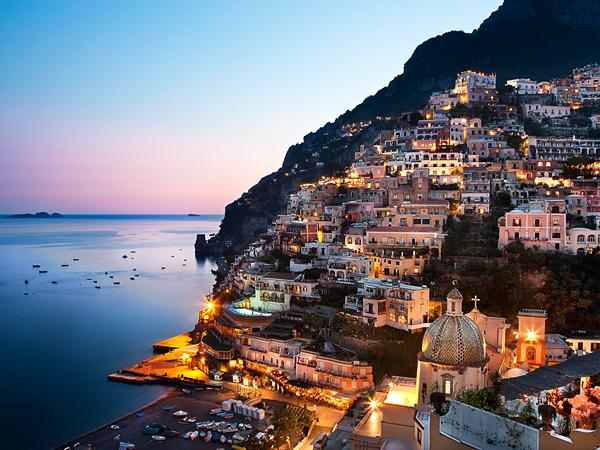
\includegraphics[scale=0.3]{../../output_images/2.1/im1_rh_100_original.jpg}
            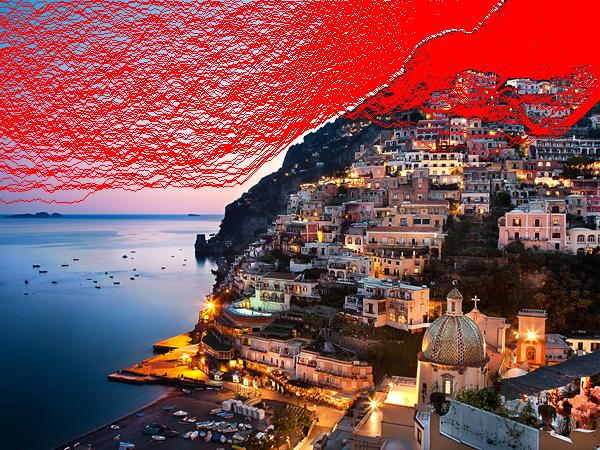
\includegraphics[scale=0.3]{../../output_images/2.1/im1_rh_100_seams.jpg}
            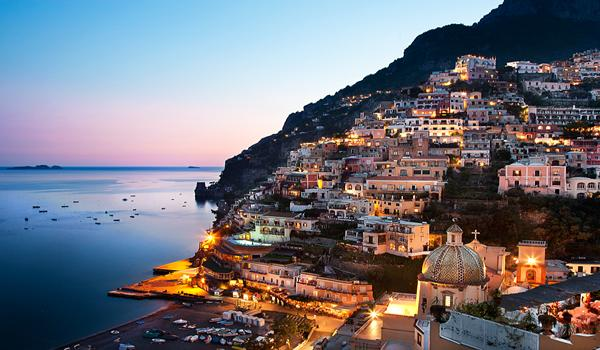
\includegraphics[scale=0.3]{../../output_images/2.1/im1_rh_100_resize.jpg}
            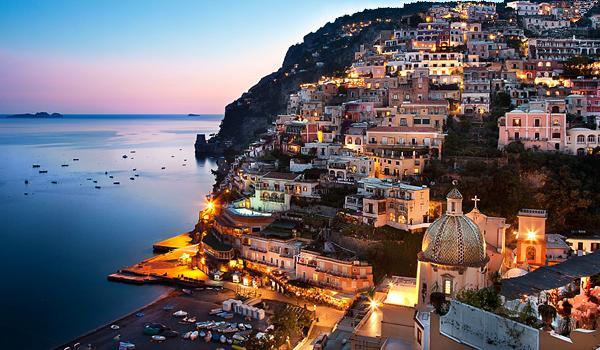
\includegraphics[scale=0.3]{../../output_images/2.1/im1_rh_100_seam_reduce.jpg}
        \end{center}
        Top left: original image1. 600 * 450 \\
        Top right: seams chosen. \\
        Bottom left: resize to 600 * 350\\
        Bottom right: seam carving reduce height to 600 * 350\\

        We could see the seams chosen are mostly pixels of sky and mountain top. And seams miss the houses in the mountain. The seam reducing keep more information than resize but it changed the shape of mountain, causing some unrealistic. \\


        For im2.jpg
        \begin{center}
            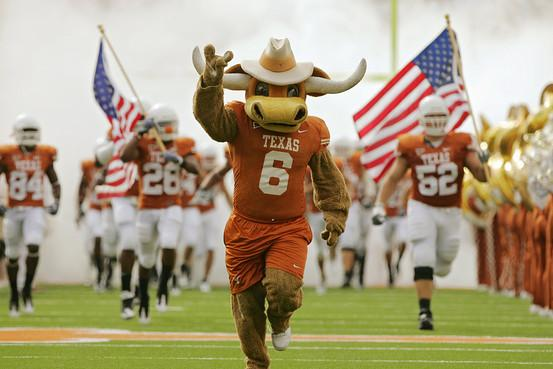
\includegraphics[scale=0.3]{../../output_images/2.1/im2_rw_100_original.jpg}
            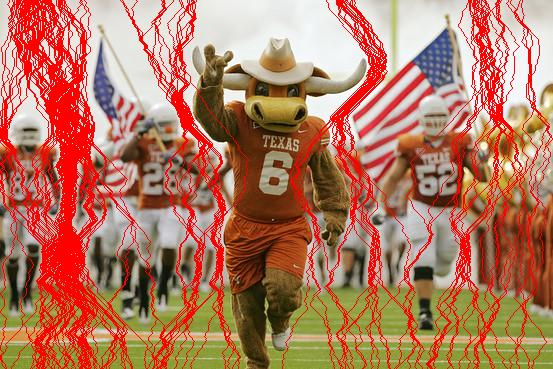
\includegraphics[scale=0.3]{../../output_images/2.1/im2_rw_100_seams.jpg}
            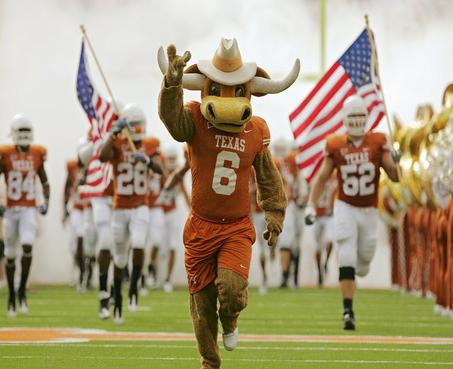
\includegraphics[scale=0.3]{../../output_images/2.1/im2_rw_100_resize.jpg}
            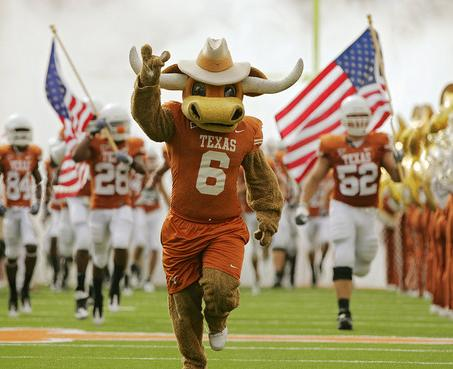
\includegraphics[scale=0.3]{../../output_images/2.1/im2_rw_100_seam_reduce.jpg}
        \end{center}
        Top left: original image2. 553 * 369 \\
        Top right: seams chosen. \\
        Bottom left: resize to 453 * 369\\
        Bottom right: seam carving reduce height to 453 * 369\\

        We could see that most of seams are in the position of interspace between people. In this example we saw seam reducing keeps the sportsman in middle of the picture more really.
\subsection{}
        \begin{center}
            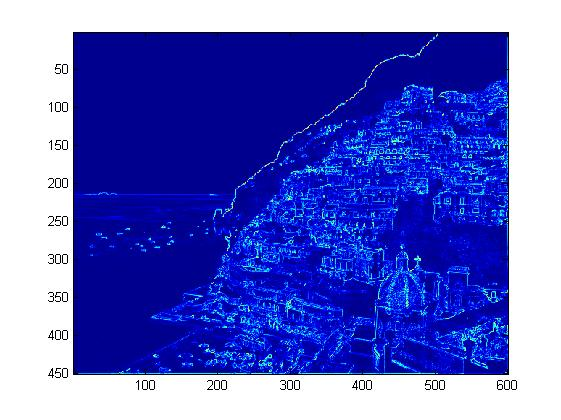
\includegraphics[scale=0.3]{../../output_images/2.2/im1_energyMap.jpg}
            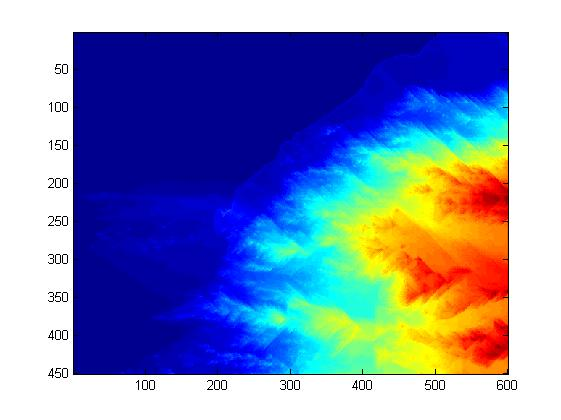
\includegraphics[scale=0.3]{../../output_images/2.2/im1_CEM_H.jpg}
            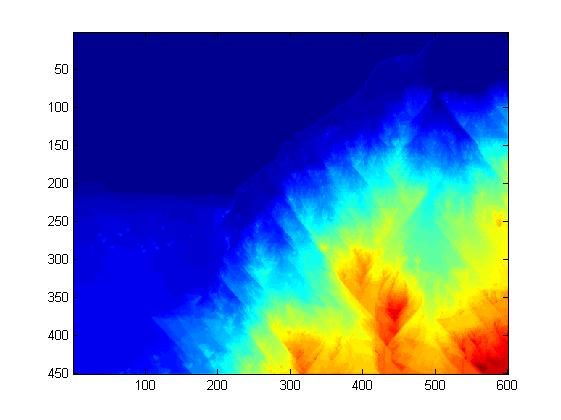
\includegraphics[scale=0.3]{../../output_images/2.2/im1_CEM_W.jpg}
        \end{center}
        Top left: energy for every piexl. \\
        Top right: cumulative energy for horizontal.\\
        Bottom: cumulative energy for vertical. \\

        Above 3 images show us the houses have more energy so the cumulative energy map has larger values in house piexls than values in sea or sky.
\subsection{}
        \begin{center}
            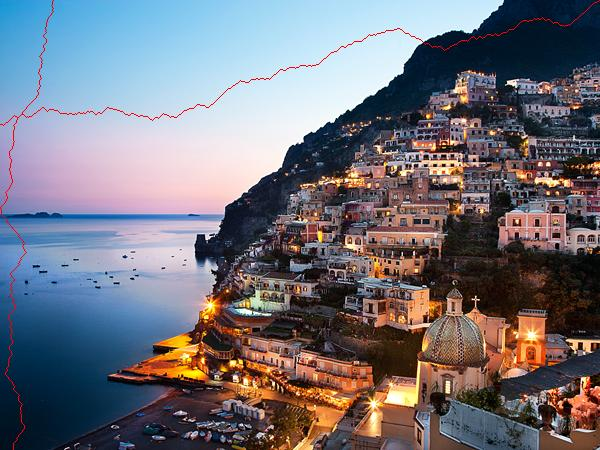
\includegraphics[scale=0.3]{../../output_images/2.3/im1_first_HV_seam.jpg}
        \end{center}
        Above image shows the first horizontal seam and vertical seam my system chosen. It passes positions without large derivative.
\subsection{}
        \begin{center}
            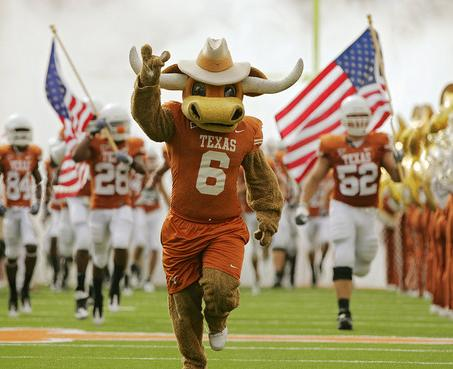
\includegraphics[scale=0.3]{../../output_images/2.4/im2_rw_diff_energy_1.jpg}
            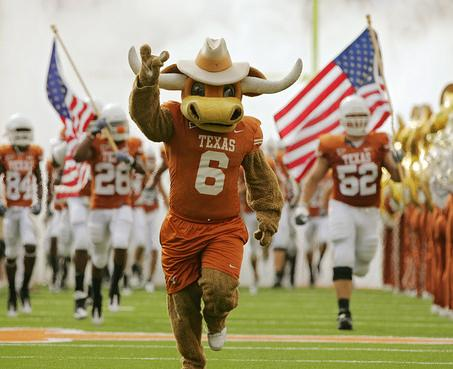
\includegraphics[scale=0.3]{../../output_images/2.4/im2_rw_diff_energy_2.jpg}
        \end{center}
        Left: energy function as $energy = |\frac{\partial I}{\partial x}| + |\frac{\partial I}{\partial y^2}|$ (im2\_rw\_diff\_energy\_1.jpg)\\
        Right: energy function as $energy = |\frac{\partial^2 I}{\partial x^2}| + |\frac{\partial^2 I}{\partial y^2}|$ (im2\_rw\_diff\_energy\_2.jpg)\\

        I used second derivative as a test energy function. The reduced images look slightly different. The people in the right image are a litter fatter.

%\end{CJK*}
\end{document}
